\documentclass[11pt]{article}
\usepackage[utf8]{inputenc}

\topmargin -.5in
\textheight 9in
\oddsidemargin -.25in
\evensidemargin -.25in
\textwidth 7in

\title{TK4 Anum : Path Calculator}
\author{Kelompok B09}
\date{May 2019}

\usepackage{graphicx}
\graphicspath{ {./img/} }
\usepackage{multicol}

\begin{document}

\maketitle

\section{Introduction}
Pada kesempatan tugas kelompok Analisis Numerik kali ini, kami mencoba untuk mengimplementasikan metode interpolasi \textit{natural cubic spline} terhadap beberapa titik koordinat yang akan diinput oleh user dengan spesifikasi tugas :

\begin{enumerate}
    \item Menginterpolasi sejumlah $n$ titik dengan kurva yang mulus (\textit{smooth}) menggunakan metode \textit{natural cubic spline}.
    \item Menghitung panjang lintasan dari detik ke-1 hingga detik ke-n.
    \item Menggambarkan kurva polinomial dari algoritma yang dipakai.
\end{enumerate}
\medskip
Setelah mengerjakan tugas ini, kami mengharapkan pengetahuan kami mengenai cara melakukan interpolasi akan semakin bertambah, terutama interpolasi dengan metode \textit{cubical spline}.

\section{Why?}
Selain sebagai tugas dari mata kuliah Analisis Numerik, kami juga mengerjakan tugas ini karena tertarik dengan bagaimana caranya interpolasi tiap titik mampu melakukan pemetaan atau \textit{plotting} lintasan kurva yang akan ditampilkan oleh komputer. Bagaimana cara menampilkan kurvanya dengan mulus tetapi bisa melewati semua titik input yang diberikan?

\section{Content}
\subsection{Aktivitas 1}

Aktivitas pertama yang kami lakukan adalah mengimplementasikan algoritma \textit{natural cubic spline} untuk bisa mendapatkan suatu kurva yang mampu melewati semua titik input tetapi juga tetap menjaga kemulusan garisnya, tidak patah - patah seperti membuat grafik garis pada umumnya. Karena interpolasi yang diminta harus berupa fungsi parametrik, maka interpolasi kami lakukan secara terpisah antara titik-titik $x$ dan titik-titik $y$ terhadap $t$. Hasil interpolasi titik-titik $x$ terhadap $t$ adalah fungsi-fungsi $x(t)$ dan hasil interpolasi titik-titik $y$ terhadap $t$ adalah fungsi-fungsi $y(t)$ yang kemudian akan menghasilkan fungsi-fungsi parametrik di tiap interval dua buah titik.

\medskip

Sama seperti metode \textit{natural cubic spline} pada fungsi biasa, pada fungsi parametrik akan dicari fungsi yang menginterpolasi titik-titik $x$ dan $y$ terhadap $t$ yang menghasilkan fungsi $(x(t),y(t))$ yang berupa \textit{piece-wise function}.

\begin{multicols}{2}
\[
    x(t) = \left\{
        \begin{array}{ll}
            x_1(t) & \quad t_1 \leq t \leq t_2 \\
            x_2(t) & \quad t_2 \leq t \leq t_3 \\
            \quad \quad \quad \quad \quad \vdots \\
            x_{n-1}(t) & \quad t_{n-1} \leq t \leq t_n \\
        \end{array}
    \right.
\]

\[
    y(t) = \left\{
        \begin{array}{ll}
            y_1(t) & \quad t_1 \leq t \leq t_2 \\
            y_2(t) & \quad t_2 \leq t \leq t_3 \\
            \quad \quad \quad \quad \quad \vdots \\
            y_{n-1}(t) & \quad t_{n-1} \leq t \leq t_n \\
        \end{array}
    \right.
\]
\end{multicols}

Di mana $x_i(t)$ adalah fungsi yang menginterpolasi titik-titik $x$ terhadap $t$ dan $y_i(t)$ adalah fungsi yang menginterpolasi titik-titik $y$ terhadap $t$ serta $t$ merupakan detik ke-$i$ posisi suatu objek berada.

\[
    x_i(t) = a_i(t-t_i)^3 + b_i(t-t_i)^2 + c_i(t-t_i) + d_i
\]

\[
    y_i(t) = a_i(t-t_i)^3 + b_i(t-t_i)^2 + c_i(t-t_i) + d_i
\]

Fungsi-fungsi $x_i(t)$ dan $y_i(t)$ bisa didapatkan dengan metode \textit{natural cubic spline} terhadap $t$.


\subsection{Aktivitas 2}

Setelah mendapatkan fungsi $(x(t),y(t))$ di aktivitas sebelumnya, selanjutnya panjang lintasan antara dua interval $t$ dapat dihitung dengan menggunakan integral dari fungsi turunan $x_i(t)$ dan $y_i(t)$.

\[
    \sum_{i=0}^{n-1} \int_{t_i}^{t_{i+1}} \sqrt{x'_i(t)+y'_i(t)} dt
\]

Untuk menyederhanakan persamaan tersebut, yang pertama kami lakukan adalah mencari turunan dari $x_i(t)$ dan $y_i(t)$ menjadi fungsi $x'_i(t)$ dan $y'_i(t)$. Pencarian turunan kami lakukan dengan menggunakan \textit{centered difference formula} dengan mengasumsikan nilai $h = 1e-11$.

\[
    x'_i(t) = \frac{x_i(t+h) - x_i(x-h)}{2h}
    \quad \quad
    y'_i(t) = \frac{y_i(t+h) - y_i(x-h)}{2h}
\]

Kemudian kami menggunakan metode pendekatan integral \textit{composite trapezoid} untuk menghitung panjang \textit{piece-wise function} di tiap interval $t$.

\[
    h \sum_{i=0}^{n-1} \frac{f(a_i) + f(a_{i+1})}{2}
\]

Untuk setiap interval $t_i$ dan $t_{i+1}$, kami mengasumsikan nilai $h = \frac{b - a}{n}$ dengan $n = 100000$, $a = t_i$, $b = t_{i+1}$. Nilai $a_i = a + ih$ dan $f(t) = \sqrt{x'_i(t)+y'_i(t)}$. Lalu setiap interval $t$ tersebut dijumlahkan untuk mendapatkan total panjang lintasannya.

\subsection{Aktivitas 3}

Setelah berhasil membuat kode dan rumus untuk interpolasi \textit{natural cubical spline} dari aktivitas 1 dan 2, pada aktivitas 3 ini kami mencoba melakukan pengetesan terhadap program kami. Program yang kami buat bisa menerima sejumlah $n$ buah sembarang titik dan membuat persamaan polinomial interpolasi berdasarkan titik - titik yang dimasukkan.

\medskip

Algoritma yang kami buat ini akan memberikan output berupa sebuah gambar kurva kartesian yang menunjukkan penggambaran kurvanya dan panjang dari kurva itu sendiri. Berikut adalah gambar kurva beserta panjang lintasan kurva tersebut terhadap n buah titik input.

\medskip

\begin{center}
Gambar 1, n = 4, panjang = 2.85265

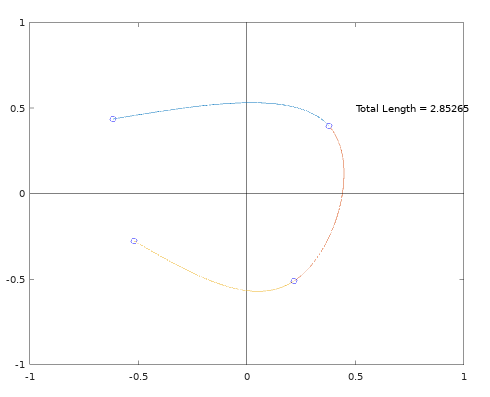
\includegraphics[width=12cm]{hasil1.png}

Gambar 2, n = 15, panjang = 5.71099

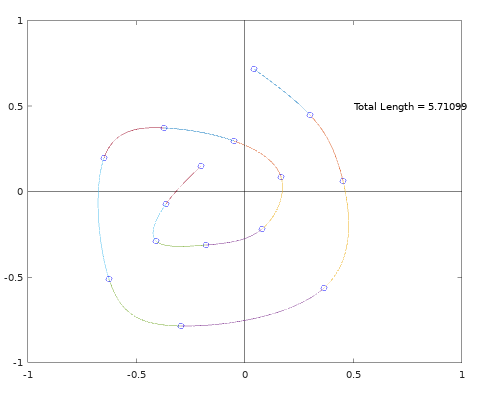
\includegraphics[width=12cm]{hasil2.png}

\end{center}

\section{Conclusion}

Setelah melakukan aktivitas 1 dan 2 serta berdasarkan hasil lintasan kurva di aktivitas 3, kami berhasil membuat algoritma \textit{natural cubical spline} yang mulus (\textit{smooth}) serta menghitung panjang dari lintasan suatu fungsi hasil interpolasi beberapa titik. Kami pun belajar hal baru berupa cara menginterpolasi fungsi parametrik dengan membuat fungsi $(x(t),y(t))$ dan menggunakan metode pendekatan integral (\textit{composite trapezoid}) untuk menghitung jarak lintasan.

\section{Reference}
\begin{enumerate}
    \item Sauer, Timothy (2012). \textit{Numerical Analysis}. Boston, MA: Pearson Education
    \item https://www.physicsforums.com/attachments/parametric-spline-tutorialv2-pdf.12898/
\end{enumerate}

\end{document}
